\documentclass[compress,9pt,xcolor={dvipsnames,table}]{beamer}
%\documentclass{beamer}
\usepackage[utf8]{inputenc}
\usepackage{lmodern}
\usepackage{textcomp}
\usepackage{algorithm}
\usepackage{algorithmic}
\usepackage{tcolorbox}
\usepackage{eurosym}
\usepackage{array}
\newcolumntype{L}[1]{>{\raggedright\let\newline\\\arraybackslash\hspace{0pt}}m{#1}}
\newcolumntype{C}[1]{>{\centering\let\newline\\\arraybackslash\hspace{0pt}}m{#1}}
\newcolumntype{R}[1]{>{\raggedleft\let\newline\\\arraybackslash\hspace{0pt}}m{#1}}


% \usepackage{polyglossia}
% \setmainlanguage{english}
\usepackage{tabularx,ragged2e}
\usepackage{booktabs}
\usepackage{dtklogos}
\usepackage{arydshln}
\usepackage{chngpage}
\usepackage{multicol}
\usepackage[caption=false]{subfig}
\hypersetup{%
  colorlinks = true,
  linkcolor  = PineGreen!100!black
}

\usepackage{natbib}

\setbeamertemplate{itemize item}{\color{PineGreen}$\bullet$}
\setbeamertemplate{itemize subitem}{\color{PineGreen!25}$\circ$}
\setbeamercolor{enumerate item}{fg=PineGreen}
\setbeamercolor{caption name}{fg=PineGreen}

% \setmainfont[]{Book Antiqua} % sets the roman font
%\setmainfont[]{Cardo}
%\setsansfont[]{PT Sans}
% \setsansfont[]{Book Antiqua} % sets the roman font
% \setmonofont[]{Consolas}
\setbeamertemplate{navigation symbols}{}
    \expandafter\def\expandafter\insertshorttitle\expandafter{%
      \insertshorttitle\hfill%
      \insertframenumber\,/\,\inserttotalframenumber}

\usetheme{Szeged}
\usecolortheme{spruce}

\title[H2020 Research and Innovation Programme]{H2020 Research and Innovation Programme}
%\author[acamacho, mgomez, rperez]{Auraham Camacho García\\Mario Alberto Gómez Rodríguez\\Rafael Pérez Torres}
\author{autor}
\institute{Cinvestav Tamaulipas}
%\date{\today}
\date{October 2015}

\begin{document}
\begin{frame}[plain]
  \begin{center}
  
\includegraphics[scale=0.12]{../../../resources/images/vectors/cinvestav-logo-no-text}
  \end{center}
  \titlepage
  
\end{frame}

%\frame{\maketitle}

\begin{frame}{Table of contents}
	\tableofcontents[hideallsubsections]
\end{frame}

\section{Introduction}
\subsection{Introduction}
\begin{frame}\frametitle{What is H2020?}
According to the official website:
\begin{quotation}
Horizon 2020 is the biggest EU Research and Innovation programme ever with nearly \EUR {80} billion of funding available over 7 years (2014 to 2020) - in addition to the private investment that this money will attract. It promises more breakthroughs, discoveries and world-firsts by taking great ideas from the lab to the market.
\end{quotation}

%The EU is conformed by 28 countries.
%[28 members, roughly 2.85 billions per country]
\end{frame}

\section{Objectives}
\label{sec:objectives}
\subsection{Objectives}

\begin{frame}\frametitle{Objectives}
Three pillars:
\begin{itemize}
    \item Excellent Science.
    \item Industrial Leadership.
    \item Societal Challenges.
\end{itemize}
Two objectives:
\begin{itemize}
    \item \emph{Spreading excellence \& widening participation}.
    \item \emph{Science with and for society}.
\end{itemize}
\end{frame}

\section{Requirements}
\subsection{Requirements}
% \begin{frame}\frametitle{Requirements}
% \begin{figure}
%         \centering
%         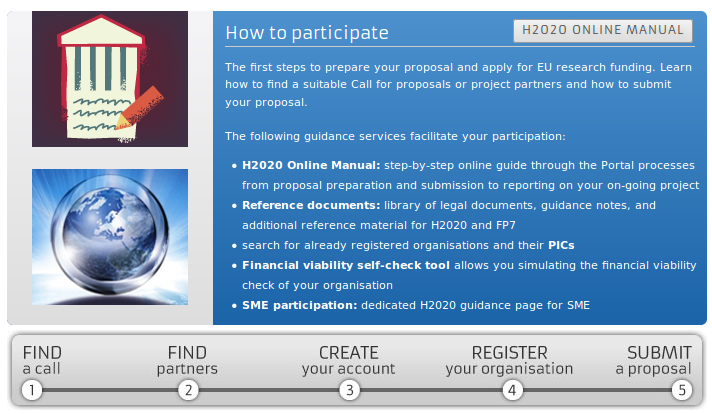
\includegraphics[width=0.8\textwidth]{images/requirements}
%         \caption{Requirements}
%         \label{fig:requirements}
%     \end{figure}
% \end{frame}

\begin{frame}\frametitle{Requirements}
The most important requirement is a \emph{full} proposal document.

A proposal consists of 2 main parts:
\begin{itemize}
  \item Administrative forms including the structured information of the basic administrative data, declarations of partners, organisations and contact persons, etc.
  \item Technical annex, which is the detailed description of the planned research and innovation project outlining work packages, costs, etc.
\end{itemize}

Proposal can be submitted multiple times, but only the last version will be evaluated.
\end{frame}

\section{Scope}
\subsection{Scope}

\begin{frame}\frametitle{H2020's scope}
Regarding  Industrial Leadership, the scope of H2020 is on:
\begin{table}
\centering
\resizebox{\textwidth}{!}{%
\begin{tabular}{@{}lr@{}}
\toprule
\multicolumn{1}{c}{\textbf{Industrial Leadership - Total funding for 2014-2020}}                                                                                           & \multicolumn{1}{c}{\textbf{\EUR{Budget}}} \\ \midrule
\begin{tabular}[c]{@{}l@{}}\textbf{Leadership in enabling and industrial technologies (LEITs)}\\ ICT, nanotechnologies, materials, biotechnology, manufacturing, space\end{tabular} & 13 557                                            \\
\begin{tabular}[c]{@{}l@{}}\textbf{Access to risk finance}\\ Leveraging private finance and venture capital\end{tabular}                                                            & 2 842                                             \\
\begin{tabular}[c]{@{}l@{}}\textbf{Innovation in SMEs}\\ Fostering all forms of innovation in all types of SMEs\end{tabular}                                                         & 616                                               \\ \bottomrule
\end{tabular}
}
\caption{Budget for Industrial Leadership pilar.}
\label{tab:budget}
\end{table}
\end{frame}

\begin{frame}\frametitle{H2020's scope}
We are focused on ICT Research and Innovation, however areas of participation for H2020 are:
\begin{multicols}{2}
\begin{itemize}
  \item Agriculture \& Forestry
  \item Aquatic Resources
  \item Bio-based Industries
  \item Biotechnology
  \item Energy
  \item Environment \& Climate Action
  \item Food \& Healthy Diet
  \item Funding Researchers
  \item Health
  \item ICT Research \& Innovation
  \item Innovation
  \item International Cooperation
  \item Key Enabling Technologies
  \item Partnerships with Industry and Member States
  \item Raw Materials
  \item Research Infrastructures
  \item Security
  \item SMEs
  \item Social Sciences \& Humanities
  \item Society
  \item Space
  \item Transport
\end{itemize}
\end{multicols}
\end{frame}

\section{Characteristics}
\subsection{Characteristics}
\begin{frame}\frametitle{A proposal's lifecycle}
% The \emph{Participant Portal} is the entry point for electronic administration of EU-funded research and innovation projects, and hosts the services for managing your proposals and projects throughout their lifecycle.
\begin{figure}
  \centering
  
\includegraphics[width=0.8\textwidth]{images/lifecycle}
  \caption{Lifecycle of a proposal}
  \label{fig:lifecycle}
\end{figure}

\begin{block}{Finding a call for proposals}
Find the most adequate call for proposals for your project idea.
\end{block}


\begin{block}{Finding partners}
Many calls require a team of at least three partners.
\end{block}

\begin{block}{Proposal's submission}
All proposals are submitted online before the deadline.
\end{block}

\end{frame}



\subsection{Proposal's lifecycle}
\begin{frame}\frametitle{Proposal's lifecycle}
\begin{block}{Evaluation}
%\begin{tcolorbox}[title=Evaluation,colframe=PineGreen]
Once the deadline has passed, all proposals are evaluated by a panel of independent specialists in their fields (five months).
The outcome of evaluation:
\begin{itemize}
  \item \textbf{0} Proposal does not meet the criterion at all or cannot be assessed due to missing or incomplete information
    \item \textbf{1 Poor}: serious weaknesses
    \item \textbf{2 Fair}: goes some way to meeting criterion, but with significant weaknesses
    \item \textbf{3 Good}: but with a number of shortcomings
    \item \textbf{4 Very good}: but with a small number of shortcomings
    \item \textbf{5 Excellent}: meets criterion in every relevant respect. Any shortcomings are minor
\end{itemize}
%\end{tcolorbox}
\end{block}
\end{frame}


\begin{frame}\frametitle{Proposal's lifecycle}    
\begin{block}{Grant agreement}
% \begin{tcolorbox}[title=Grant agreement,colframe=PineGreen]
The European Commission then draws up a grant agreement with each participant, confirming the research \& innovation activities that will be undertaken, the project duration, budget, rates and costs, the European Commission's contribution, all rights and obligations and more.
The time limit for signing the grant agreements is generally \textbf{three months}.
% \end{tcolorbox}
\end{block}

\end{frame}

\section{Range of funding}
\subsubsection{Range of funding}
\begin{frame}\frametitle{Range of funding}
\begin{table}
\centering
\resizebox{\textwidth}{!}{%
\begin{tabular}{C{0.2\linewidth}C{0.05\linewidth}C{0.2\linewidth}C{0.15\linewidth}C{0.15\linewidth}C{0.3\linewidth}C{0.5\linewidth}}
%\begin{tabular}{lllllll}
\toprule
\textbf{Type of action} & \textbf{Code} & \textbf{Minimum conditions} & \textbf{Funding} & \textbf{Typical duration} & \textbf{Average EC contribution} & \textbf{Aim} \\ 
\midrule
Research \& Innovation Action & RIA & $\geq$ 3 legal entities from 3 MS/AC & 100\% & 36-48 months & \EUR{2.0 - 5.0 M} & Collaborative research projects \\
\cmidrule{1-7}
Innovation Action                           & IA                                & $\geq$ 3 legal entities from 3 MS/AC                & 70\%                                             & 30-36 months                                         & \EUR{2.0 - 5.0 M}                                                                                                 & produce plans \& arrangements or designs for new, altered or improved products, processes or services           \\

\cmidrule{1-7}
Coordination \& Support Action              & CSA                               & 1 legal entity                                  & 100\%                                            & 12-30 months                                         & \EUR{0.5 - 2.0 M}                                                                                                     & Accompanying measures (standardisation, dissemination), no research                                             \\

\cmidrule{1-7}
ERC Grants                                  & ERC                               & 1 legal entity in MS/AC                         & 100\%                                            & 60 months                                            & \begin{tabular}[c]{@{}l@{}}Starting: $\leq$ \EUR{2.0 M}\\ Consolidator: $\leq$ \EUR{2.75 M}\\ Advanced: $\leq$ \EUR{3.5 M}\end{tabular}       & Support excelent investigators and their research teams to pursue ground-breaking, high-gain/high-risk research \\

\cmidrule{1-7}
SME Instrument                              & SME                               & 1 SME in MS/AC                                  & \multicolumn{3}{l}{\begin{tabular}[c]{@{}l@{}}3 phases: \\ - Phase 1. lump sum of \EUR{50 K} per project\\ - Phase 2: \EUR{1 - 2.5 M} per project (1-2 years), \\70\% of eligible costs reimbursed\\ - Phase 3: no funding\end{tabular}} & Combination of demonstration activities (testing, prototyping), market replication                              \\

\cmidrule{1-7}
Fast Track to innovation                    & FTI                               & $\leq$ 5 legal entities from 5 MS/AC               & 70\%                                             & -                                                    & $\leq$ \EUR{3.0 M}                                                                                                       & Produce plans \& arrangements or designs for new, altered or improved products, processes or services           \\
\bottomrule
\end{tabular}
}
\caption{Fundings per type of action}
\label{tbl:fundings}
\end{table}
\end{frame}


\section{Expected results}
\subsubsection{Expected results}
\begin{frame}\frametitle{Expected results}
\begin{itemize}
  \item Expected results depend on the specific call for proposals and context of the project.
  \item Nevertheless, it is stated that \textbf{open access} must be granted to all scientific publications resulting from Horizon 2020 actions, and proposals must refer to measures envisaged.
  \item In order to receive fundings, periodically some deliverable artifacts should be presented, like information, special report, a technical diagram brochure, list, a software milestone or other building block of the action.
\end{itemize}
\end{frame}

\subsection{Mexican participation}
\begin{frame}\frametitle{Mexican participation}
\begin{itemize}
  \item Horizon 2020 is open to participation from across the world.
  European researchers can include partners from anywhere in the world when preparing H2020 proposals.
  \item This means that Mexican researchers, enterprises and institutions can team up with their European partners to participate in projects under H2020.
  \item However, Mexican partners are not automatically eligible for funding through H2020.
  \item Mexico created in February 2014 a complementary funding mechanism called CONACYT-Horizon 2020 providing a source of financing ``project-by-project participation'' to Mexican partners in successful H2020 projects covering all thematic areas
\end{itemize}
\end{frame}


\end{document}